\documentclass[12pt]{amsart}
\pagestyle{empty}

\textheight=9.5in   \voffset=-1in
\textwidth=7in      \hoffset=-1in

\usepackage{latexsym,tikz,calc}

\parindent 0in
\parskip \baselineskip

%%%%%%%%%%%%%%%%%%%%%%%%%%

\begin{document}
\thispagestyle{empty}
%%%%%%%%%%%%%%%%%%%%%%%%%%
\centerline{\large Exam  \hfill Math 122 Sections 1 and 2 Fall 2012 \hfill Name: \underline{\phantom{Your name goes here, }}} 
 

 \indent \textbf{Directions:}\\
	\indent \indent 1) Each question is worth 5 points (for a total of 150 points)\\
	\indent \indent 2) Calculators are allowed, but all cell phones/PDA devices must be put away.\\ \indent \indent \ \ \ \ No calculator sharing.\\
	\indent \indent 3) Show all work for full credit.\\
	\indent \indent 4) Read all directions carefully and clearly indicate your final answer.\\
	\indent \indent 5) Round any approximate answers to \textbf{3 decimal places}.\\
 

\begin{enumerate}
\item %1

Using the table of values for the  function $f(x)$

\centerline{\begin{tabular}{|c|c|c|c|c|c|c|c|c|}
\hline
 $x$&1&2&3&4&5&6&7&8\\
\hline $f(x)$&2.3&2.8&3.2&3.7&4.1&5.0&5.6&6.2\\
\hline
\end{tabular}}

\vspace{.2in}

 

answer the following :

 \vspace {.3in}
 
What is $f(7)$?  \underline{\hspace {1in}}
  
 \vspace {.3in}
 
 What is the value of $x$ when $f(x)=2.3$?   \underline{\hspace {1in}}
 
 \vspace {.3in}
 
What is the average rate of change of $f$ between $x=2$ and $x=5$?     \underline{\hspace {1in}}

\vspace{.3in}

\item %2

Let $f(x)=-x^3+x^2+6x$.  Where is this function increasing?

\vspace{.5in}

\item %3
Find the slope of a line perpendicular to the line passing through the points $(-1,2)$ and $(3,7)$.

\vspace{.65in}

\item %4

An object is put outside on a cold day at time $t=0$. Its temperature $H=f(t)$ at time $t$ (in minutes) is given in degrees $^{\circ} C$.  
What does the statement $f(30)=10$ mean in terms of temperature?  Include units for $30$ and $10$ in your answer.

\vspace{.8in}

\item %5
Let $f(x)= x^2-3x+4$ and $g(x)=\dfrac{x}{2}+8$.

\vspace{.3in}

Find $f(x)-g(x)$:   $f(x)-g(x) =$\underline{\hspace {1in}}

\vspace{.3in}

Find $f(g(-8))$.  Show work:      $f\big( g(-8)\big) = $ \underline{\hspace {1in}}

\vspace{.3in}

\item %6
A deposit is made into an interest bearing account.  The graph shows the balance $B$ in the account $t$ years later.  Find the equation of the graph---you many assume the interest rate is compounded continuously.  Note that $B=2000$ at time $t=0$ and that $B=7000$ after 20 years.

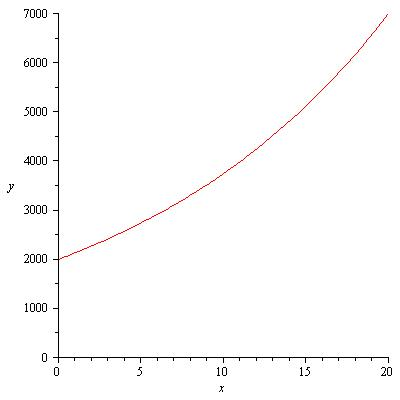
\includegraphics [width=2.25in]{graphpbm6ex}

\item %7 
Solve for $x$ using logarithms.

$3^{5x}=100$

\vspace{.5in}

\item %8
Find a linear equation for $y=f(x)$ if $f(2)=7$ and $f(-6)=-5$.

\vspace{1in}

\item %9
How long will it take 50 grams of a substance to decay to 10 grams if the continuous rate of decay is $k=-0.345$ where time is measured in years?


\vspace{.8in}


\item %10
The table below shows world gold production $G=f(t)$ as a function of the year $t$.

\vspace{.25in}

\centerline{\begin{tabular}{|c|c|c|c|c|c|}
\hline
 $t$ (year)&1990&1993&1996&1999&2002\\
\hline $G$ (mn troy ounces)&70.2&73.3&73.6&82.6&82.9\\
\hline
\end{tabular}}

\vspace{.25in}

Estimate $f^{ \prime}(1996)$.     \underline{\hspace {1in}}

\vspace{.3in}

Give units and interpret your answer in terms of gold production.

\vspace {.5in}

\item %11

The number of bacteria after $t$ hours in a laboratory experiment is given by $n=f(t)$.

What are the units of the derivative $f^{\prime}(t)$?


\vspace {1in}

\item %12 
A graph of $f(x)$ is given below.  Sketch the derivative $f^{ \prime}(x)$.

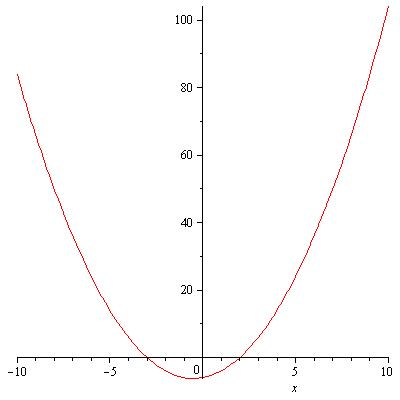
\includegraphics [width=2.25in]{graphpbm11ex}

\vspace {.3in}


\item %13

Find the equation of the line tangent to the graph of $y=80t-16t^2$ at $t=3$.

\vspace{1in}



Find the following derivatives:

\item %14
$y=x^4+8x^2-2x+4 \qquad y'=$\underline{\hspace {1in}}

\vspace{.5in}

\item %15 
$f(x)=5\ln x \qquad f'(x)=$ \underline{\hspace {1in}}

\vspace{.5in}

\item %16
$g(x)=e^{2x} \qquad g'(x)=$\underline{\hspace {1in}}

\vspace{.5in}

\item %17 
$y=\sqrt{x^4+1} \qquad y'=$\underline{\hspace {1in}}

\vspace{.5in}

\item %18
$f(x)=\dfrac{e^{2x}}{x^2+1} \qquad f'(x)=$\underline{\hspace {1in}}

\vspace{.5in}

\item %19
$f(x)=x^2 \ln x \qquad f'(x)=$\underline{\hspace {1in}}

\vspace{.5in}

\item %20

Find the global minimum for $f(x)=x^{10}-10x$  for $0\leq x\leq 2$

\vspace{.8in}

\item %21

 100 fish are released in a small pond. The rate of growth of
the number of fish, $r(t)$, is given by:

    \centerline{
      \begin{tabular}{|c|c|c|c|c|}
	\hline
	$t$ (time in weeks) & 0 &2 & 4 & 6\\ \hline
	$r(t)$ (fish per week)& 15 & 17 & 21 & 23 \\ \hline
      \end{tabular}
    }
    
     \vspace{.25in}
     	Use a left hand sum to estimate the number of fish after 6  
 		weeks.                  \underline{\hspace {1in}}  
 		
 		\vspace{.3in}
		Use a right hand sum to estimate the number of fish after 6  
 		weeks.    \underline{\hspace {1in}}
 		\vspace{.3in}
		
		Give an good guess for the number of fish after 6  
 		weeks.  
		\underline{\hspace {1in}}
		\vspace{.5in}

		
		
		\item %22
		
		Compute the following definite integrals:
		\vspace{,2in}
		
		$\displaystyle \int_0^2 xe^x\, dx =$          \underline{\hspace {1in}}
		
		\vspace{.3in}
		
		$\displaystyle\int_1^4x\sqrt{x^2+1}\, dx=$       \underline{\hspace {1in}}
		
		\vspace{.3in}
		
		\item %23
		
		Find the following antiderivatives:
		
		
		$\int x^3+4x+8\, dx=$          \underline{\hspace {1in}}
		
		\vspace{.3in}
		
		$\int\frac{5}{x}\,dx=$       \underline{\hspace {1in}}
		
		\vspace{.3in}
		
		\item %24
		Integrate by substitution:
		
		$\int x(x^2+9)^6\, dx=$       \underline{\hspace {1in}}
		
		\vspace{.5in}  

\item %25 

Use the Fundamental Theorem of Calculus to evaluate the integral
$\displaystyle \int_0^1e^{-0.2t}\, dt$       		
		\vspace{.5in}
		
	\item % 26
	
	If $f(t)$ is measured in inches per minute and $t$ is measured in minutes, what are the units of $\int f(t)dt$?     \underline{\hspace {1in}}
		
		\vspace{.5in}

	
		
		\item %27
		
		Find an antiderivative $F(x)$ of  $F^{\prime}(x)=x^3-3$  with
the added condition that $F(2)=8$ .
		
		\vspace{1in}

				
		\item  %28
		Given the following graph of the \underline{derivative} $F^{\prime}(x)$ sketch a possible graph for $F(x)$.
		
		\vspace{.3in}
		
		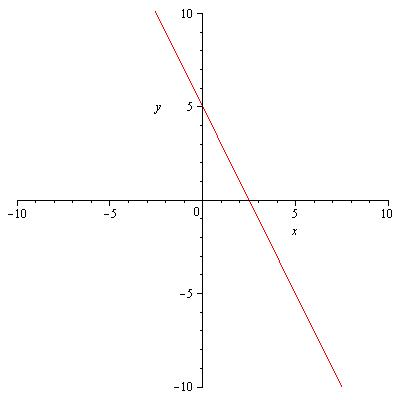
\includegraphics [width=2.25in]{graphpbm28ex}
		
			\vspace{.3in}
			
		
		\item %29
		
		Find the area between the curves: $y=x^2$ and $y=x+6$.  These functions are graphed below. Shade the area you have been asked to find.
		
			\vspace{.3in}
			
		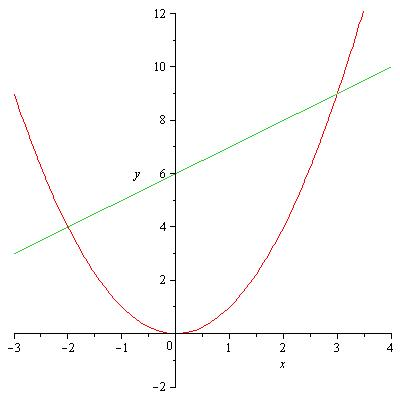
\includegraphics [width=2.25in]{graphpbm29ex}
		
		\vspace{.3in}
	
			Area=\underline{\hspace {1in}}
		
		\vspace{.5in}


\item %30
\  The rate that water is pumped into a tank is $r(t)=6-5(.9)^t$
gallons per minute where $t$ is the time in minutes since the pumping
started.  
     
     	\vspace{.3in}
	
     	What are the units on $\displaystyle 
        \int_0^{30}r(t)\,dt$\ ?
        
    	\vspace{.3in}
	


	 How much water was pumped into the tank in the first 30
     minutes?
     
     	\vspace{.3in}
	

        
     









\end{enumerate}
\end{document}
